\section{Escenarios de Estudio}

En esta sección se describe las distintas escenas y configuraciones a realizar para las distintas pruebas sobre la aplicación.

\subsection{Escenas de Prueba y Objetos}

Para la realización de pruebas de precisión y rendimiento se utilizan siete escenas las cuales se clasifican en dos categorías: escenas completas y ambientes de pruebas llamados escenas \emph{sandbox}. Todas las escenas comprenden varios niveles de complejidad con respecto a geometría e iluminación. La aplicación también incluye una serie de modelos precargados los cuales serán agregados a las escenas, estos objetos son considerados dinámicos.

\subsubsection{Escenas Completas}

Como escenas completas se consideraron cuatro escenas comunes para pruebas de iluminación global. Estas escenas presentan varios niveles de complejidad geométrica y de propagación de luz. En la Tabla \ref{tab:scenes_attributes} se listan sus nombres y atributos.

\begin{table}[h]
\centering
\begin{tabular}{|l|l|l|l|l|l|}
\hline
Nombre            & Vértices & Triángulos & Texturas & Geometría & Iluminación \\ \hline
Sponza     & 153.635  & 278.163    & Sí       & Compleja  & Compleja     \\ \hline
Conference   & 194.399  & 331.179    & No       & Compleja  & Compleja     \\ \hline
Sibenik & 40.479   & 75.283     & Sí       & Media     & Media        \\ \hline
Cornell Box       & 72       & 36         & No       & Simple    & Simple       \\ \hline
\end{tabular}
\caption{Escenas completas y sus atributos.}
\label{tab:scenes_attributes}
\end{table}

\paragraph{Sponza:} Modelo del atrio del palacio Sponza en Dubrovnik. Este modelo originalmente realizado por Marko Dabrovic y luego remodelado por Frank Meinl de Crytek con nuevos elementos como cortinas, vasos y plantas, además de mapas especulares, albedo y normales \cite{sponza_model}. Esta es una escena de dimensión considerable con propagación de luz compleja, especialmente en las áreas ocluidas por las cortinas y los pasillos superiores donde la luz difusa rebota luego de pasar a través de varias columnas. En la Figura \ref{fig:crytek_sponza} se puede observar esta escena.

\begin{figure}[H]
	\centering
	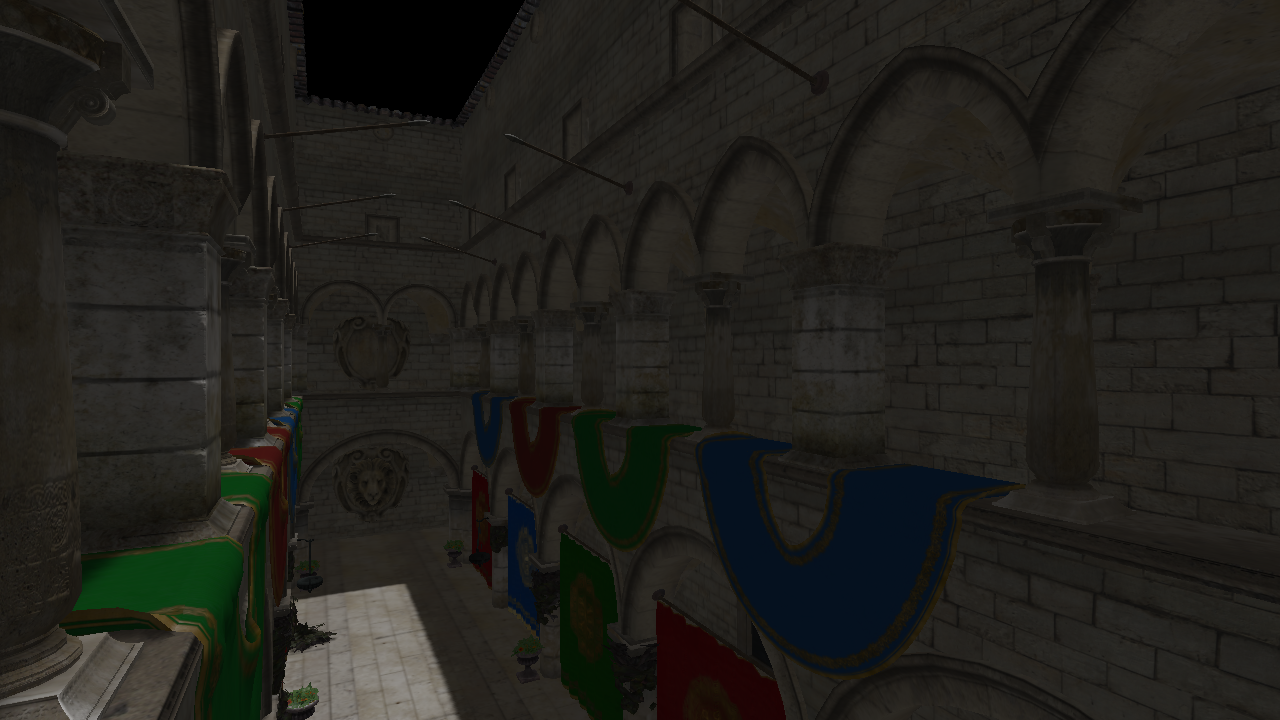
\includegraphics[width=0.65\linewidth]{media/scenes/sponza.png}
	\caption{Sponza con solo iluminación directa desde una luz direccional más luz ambiental para visualizar las áreas sombreadas.}
	\label{fig:crytek_sponza}
\end{figure}

\paragraph{Conference:} Un modelo 3D basado en una sala de conferencias del \emph{Lawrence Berkeley National Laboratory} \cite{conference_model}. Esa es una escena interior pequeña pero de gran complejidad geométrica con muchos objetos similares. El transporte de luz es particularmente complejo en ciertas partes como debajo de sillas o la mesa central. En la Figura \ref{fig:conference} se puede observar esta escena.

\begin{figure}[H]
	\centering
	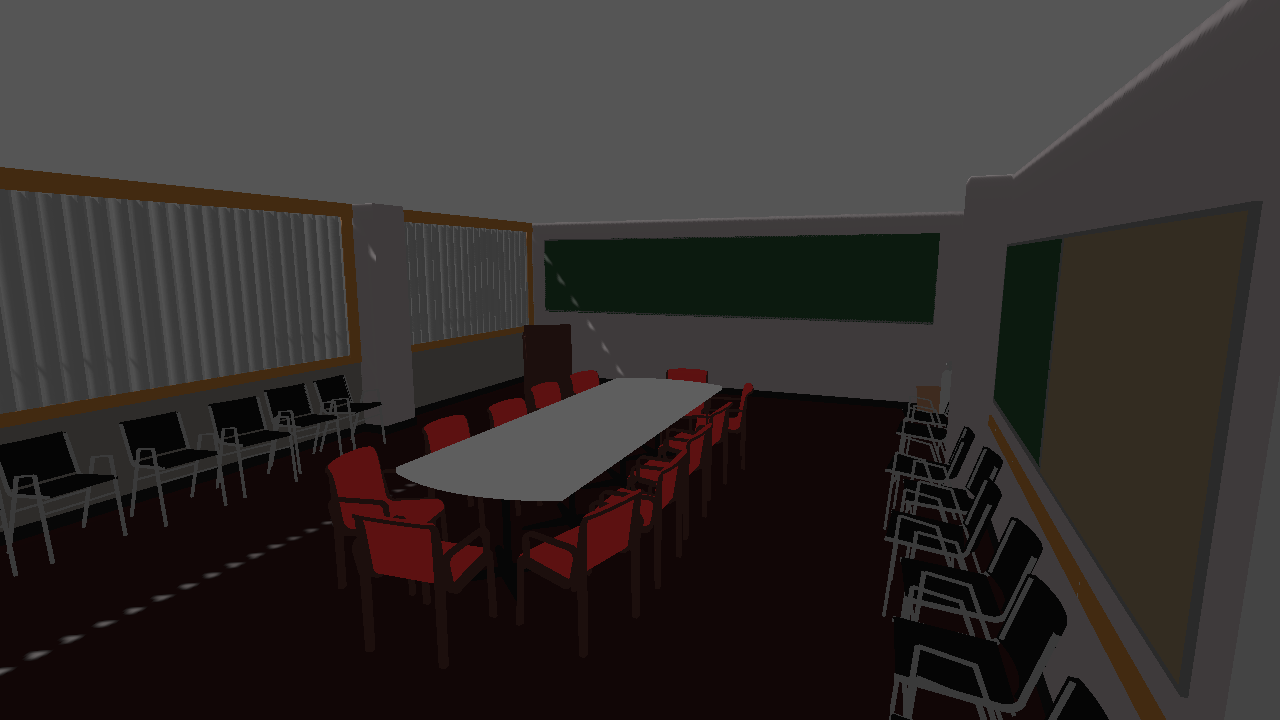
\includegraphics[width=0.65\linewidth]{media/scenes/conference.png}
	\caption{Conference con solo iluminación directa desde una luz direccional más luz ambiental para visualizar las áreas sombreadas.}
	\label{fig:conference}
\end{figure}

\paragraph{Sibenik:} El interior de una catedral \cite{sibenik_model}. La luz entra a ella a través de ventanas y se propaga por toda la escena. La escena tiene una sección con columnas ideal para probar sombras. En esta misma sección de columnas hay un piso de mármol que permite apreciar reflexión especular. Una alfombra roja cubre gran parte de la catedral esta permite la visualización de reflexión difusa. En la Figura \ref{fig:sibenik} se puede observar esta escena.

\begin{figure}[H]
	\centering
	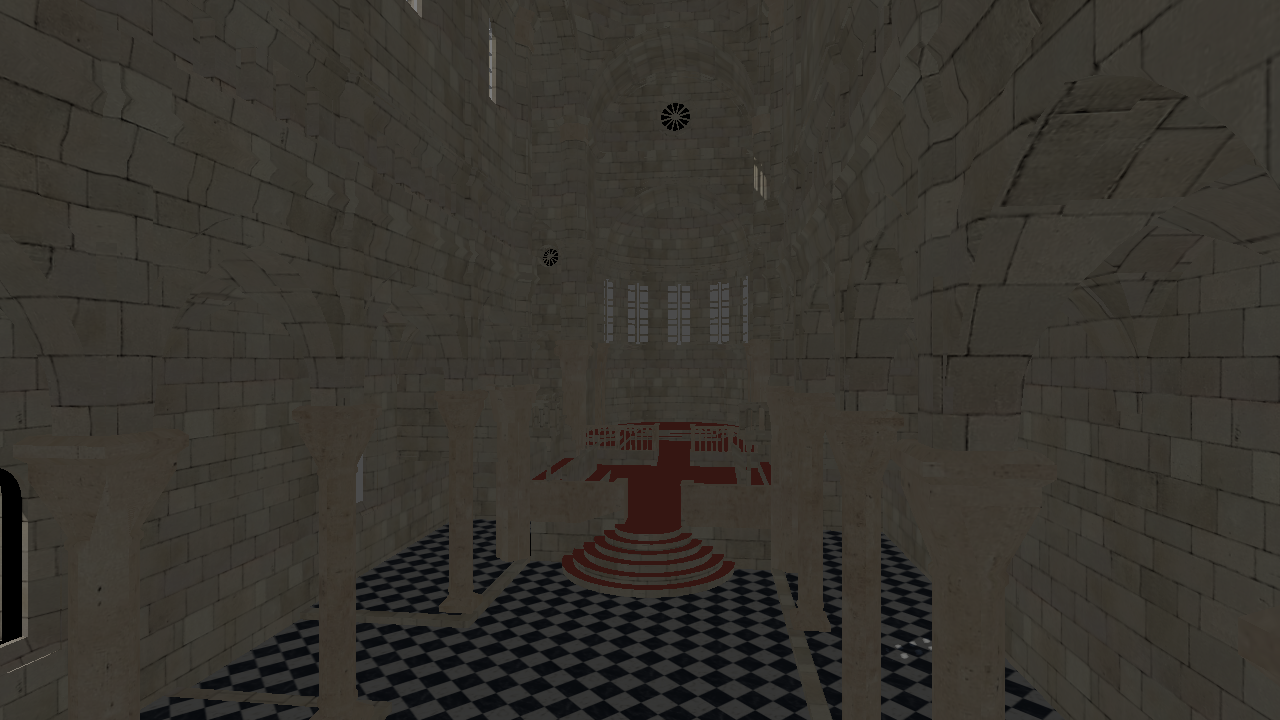
\includegraphics[width=0.65\linewidth]{media/scenes/sibenik.png}
	\caption{Sibenik con solo iluminación directa desde una luz direccional más luz ambiental para visualizar las áreas sombreadas.}
	\label{fig:sibenik}
\end{figure}

\paragraph{Cornell Box:} Este es un modelo para la visualización de iluminación global. Creado por Donald Greenberg y estudiantes de \emph{Cornell University} \cite{cornell_model}. El Cornell Box está compuesto por una caja con dos paredes de colores, a la izquierda una roja y a la derecha una verde, el resto de la caja es blanca. Dentro de esta caja se encuentran dos cajas más, una pequeña y otra más alta. En la Figura \ref{fig:cornell} se puede observar esta escena.

\begin{figure}[H]
	\centering
	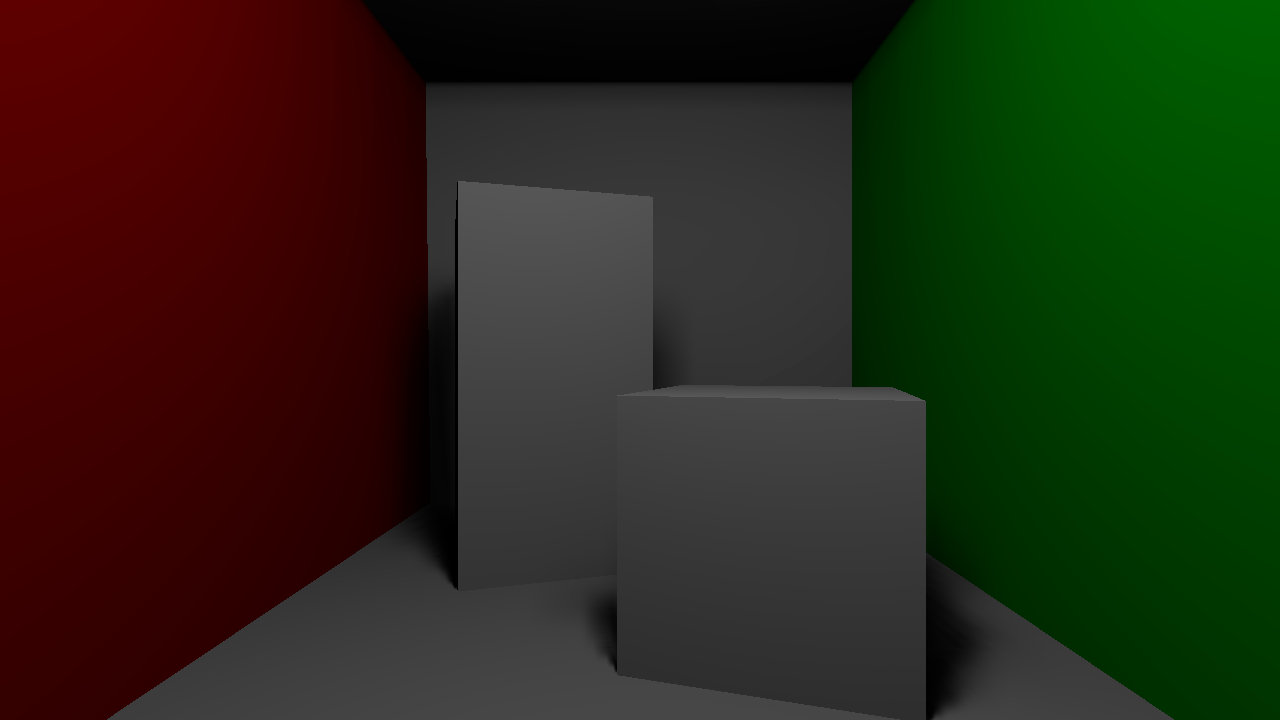
\includegraphics[width=0.65\linewidth]{media/scenes/cornell.png}
	\caption{Cornell Box con solo iluminación directa desde una luz puntual con trazado de sombras.}
	\label{fig:cornell}
\end{figure}

\subsubsection{Escenas Sandbox}

Las escenas sandbox son entornos simples y vacíos donde se realizaran pruebas de aspectos específicos de la aplicación. Estas escenas no presentan mayor complejidad geométrica o complejidad de iluminación. En la Tabla \ref{tab:sandbox} se listan sus nombres y atributos.

\begin{table}[h]
\centering
\begin{tabular}{|l|l|l|l|l|l|}
\hline
Nombre            & Vértices & Triángulos & Texturas & Geometría & Iluminación \\ \hline
Light Box         & 4.098    & 8.192      & No       & Simple    & Simple        \\ \hline
Plane Test        & 16       & 24         & No       & Simple    & Simple       \\ \hline
Cornell Box Vacío & 24       & 12         & No       & Simple    & Simple       \\ \hline
\end{tabular}
\caption{Escenas Sandbox y sus atributos.}
\label{tab:sandbox}
\end{table}

Light Box es un interior donde los bordes son tan suaves que no hay oclusión ambiental, el interior es totalmente blanco y no hay cambios bruscos en geometría, esto maximiza la propagación de luz en esta escena. Plane Test es sencillamente un plano, en una esquina se encuentra un cuboide fino pero de gran altura para permitir la voxelización de objetos sobre el plano. Cornell Box Vacío es la escena completa Cornell Box sin las cajas internas. En la Figura \ref{fig:sandboxscenes} se puede observar todas las escenas sandbox.

\begin{figure}[H]
	\centering
	\begin{subfigure}[t]{0.32\textwidth}
		\centering
		\captionsetup{justification=centering}
		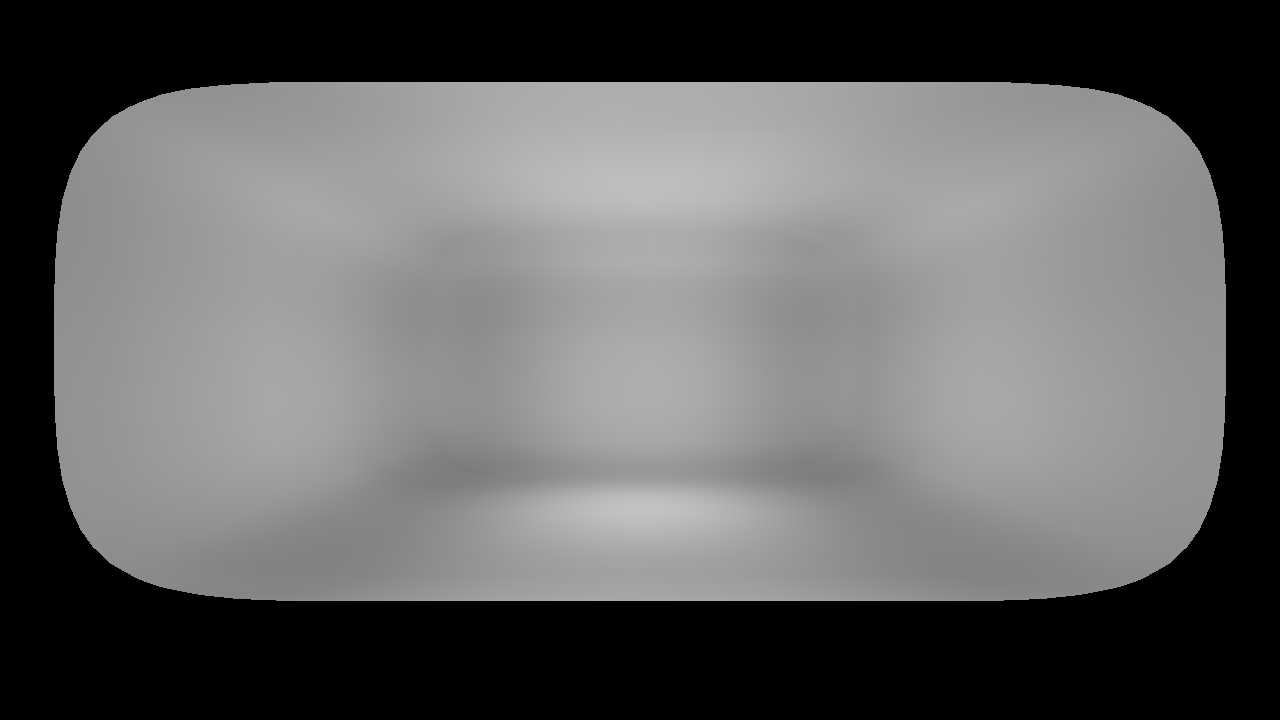
\includegraphics[width=\linewidth]{media/scenes/lightbox.png}
		\caption*{Escena Light Box con solo iluminación directa desde una luz puntual de baja intensidad.}
	\end{subfigure}%
		\hspace{0.01\textwidth}
	\begin{subfigure}[t]{0.32\textwidth}
		\centering
		\captionsetup{justification=centering}
		
\includegraphics[width=\linewidth]{media/scenes/plane.png}
		\caption*{Escena Plane Test con solo iluminación directa desde una luz direccional.}
	\end{subfigure}%
		\hspace{0.01\textwidth}
	\begin{subfigure}[t]{0.32\textwidth}
		\centering
		\captionsetup{justification=centering}
		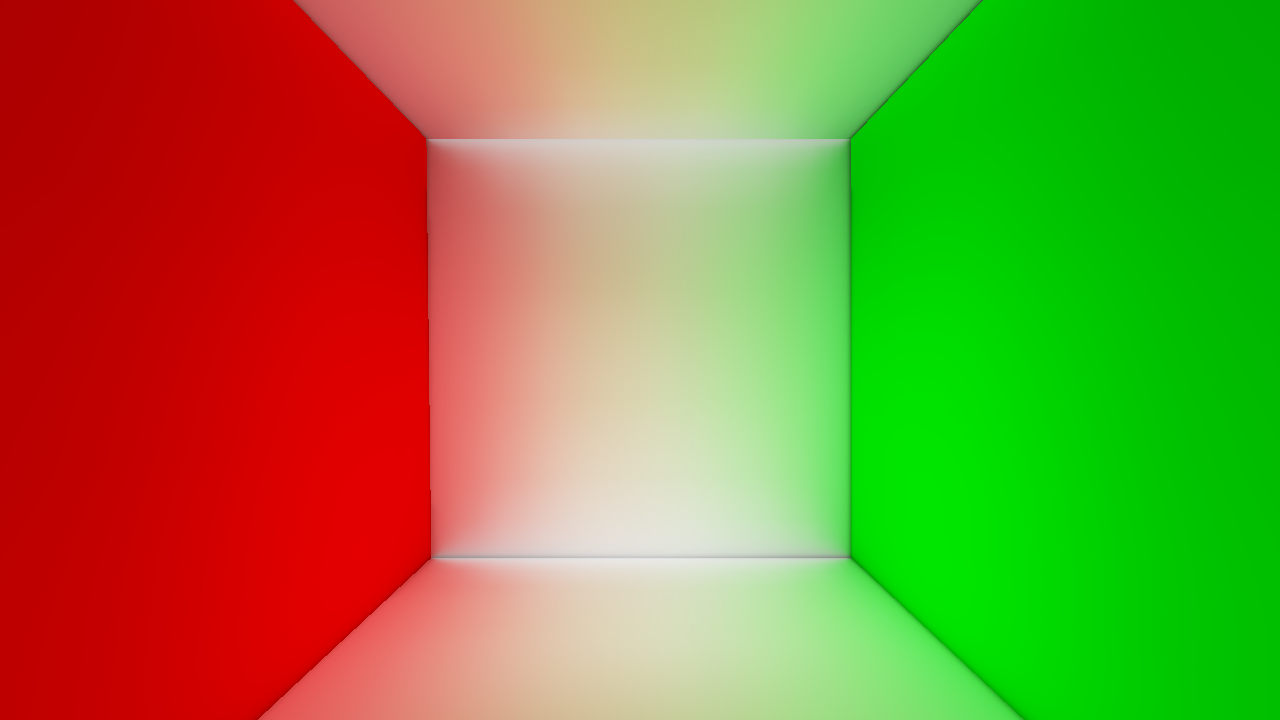
\includegraphics[width=\linewidth]{media/scenes/cornell_empty.png}
		\caption*{Escena Cornell Box Vació con iluminación indirecta y solo una luz puntual.}
	\end{subfigure}
	\caption{Escenas sandbox.}
	\label{fig:sandboxscenes}
\end{figure}

\subsubsection{Objetos Precargados}
La aplicación cuenta con una serie de objetos tridimensionales que pueden ser agregados a las escenas. Cada uno de estos objetos puede tener su propio material y matriz espacial. Estos objetos son considerados dinámicos por la aplicación. Los objetos están divididos en dos categorías: primitivas y modelos. Las primitivas son: Icosaedro, Cubo, Esfera, Cono, Toro, Plano y Cilindro. Los modelos son: Stanford Happy Buddha, Stanford Bunny, Stanford Dragon y Utah Teapot. En la Figura \ref{fig:models} se puede observar todos estos objetos.

\begin{figure}[H]
	\centering
	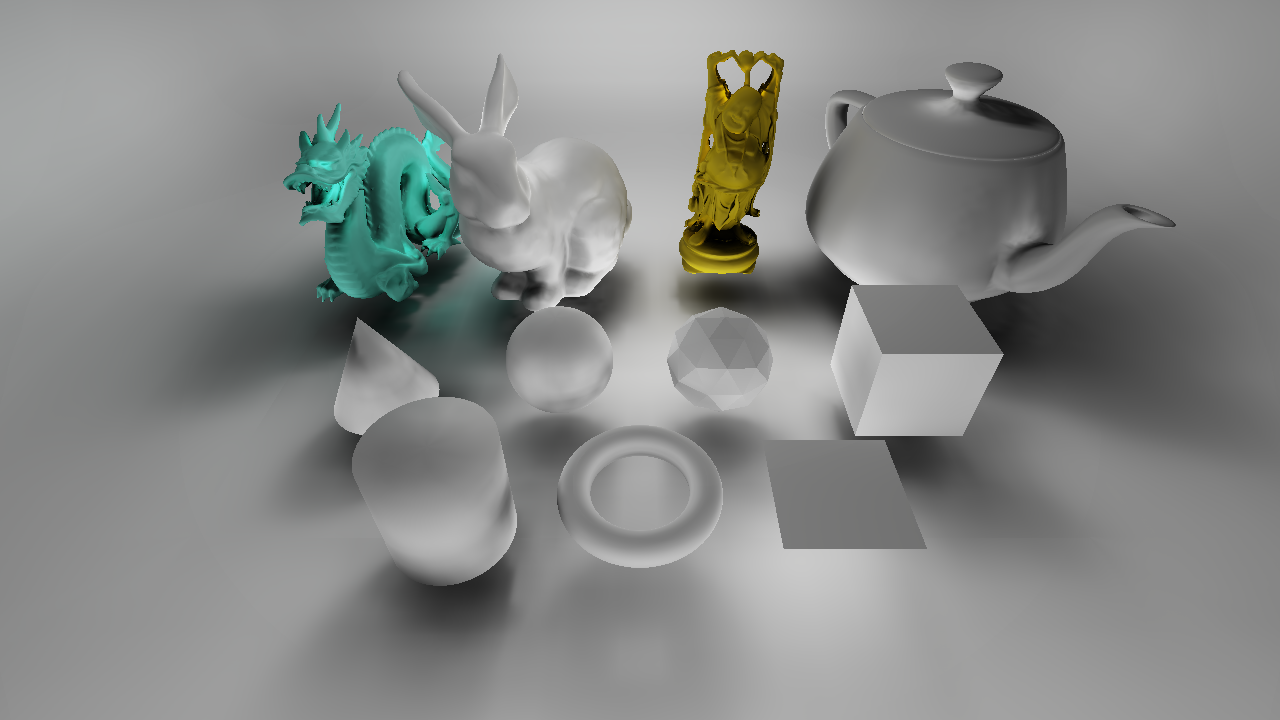
\includegraphics[width=0.95\linewidth]{media/scenes/models.png}
	\caption{Objetos precargados. Arriba se encuentra los modelos Stanford Dragon, Stanford Bunny, Stanford Happy Buddha y Utah Teapot. El resto son primitivas, de izquierda a derecha: Cono, Esfera, Icosaedro, Cubo, Cilindro, Toro y Plano. Todos los objetos se encuentra en la escena Light Box utilizando una luz focal con trazado de sombras e iluminación indirecta.}
	\label{fig:models}
\end{figure}

\subsubsection{Criterios de Complejidad Geométrica e Iluminación}

Para determinar la complejidad geométrica de cada escena se consideró la cantidad de triángulos que estas poseen y no la cantidad de objetos a renderizar ya que este es el factor que mayor afecta el proceso de voxelización.

Para determinar la complejidad de iluminación se consideraron los siguientes aspectos:

\begin{enumerate}
	\item El nivel de detalle de la representación en vóxeles de la escena. En la escena Cornell Box la representación en vóxeles es muy similar a la geometría original. En contraste la escena Sponza difiere considerablemente de la geometría original en lugares con detalles finos como los vasos y plantas de esta escena.
	\item Secciones ocluidas y facilidad de propagación de luz sobre distintas áreas de la escena. En la escena Cornell Box la luz se propaga fácilmente desde cualquier superficie iluminada a otras partes de la escena. En contraste escenas como Conference o Sponza tienen complicadas secciones de geometría como las sillas en Conference y las cortinas inferiores en Sponza que reducen la luz a pequeños haces.
\end{enumerate}
